%TODO 
% 1) Add the new robot design 

\chapter{Clothing Robots}
This chapter describes the design of Rovables, small robots that can move on the clothing. 

\section{Introduction}
The design and implementation of Rovables were guided by the following  considerations: 
\begin{enumerate}
\item \textbf{Small form-factor}. The devices should be as small and as lightweight as possible. Since the device is close to the body, smaller size and weight is less obtrusive for the human host. Furthermore, clothing has limited space for travel, especially places such as sleeves. The size should be limited to 1.5cm x 1.5cm, the diameter of a small wristwatch.    

\item \textbf{Navigation}
The robot should be able to track its positions on unmodified clothing. Such a system should not require external aids, such as cameras. This will allow autonomous movement on the host's clothing, without disturbing or limiting the wearer.

\item \textbf{Mobility}
The device should move freely vertically on unmodified clothing. Furthermore, it should be able to move on loose and wrinkled clothing. The device should be able to carry a payload, allowing it to actuate clothing or to carry sensors. 

\item \textbf{Communications} 
The device's basic functionality should include wireless communications with external devices. This will allow coordination between multiple robots and interaction with devices such as PCs and mobile phones. Communications between robots will enable more complex behavior and tasks. 

\item \textbf{Power} 
As manually charging multiple robots can be time-consuming, the robot should have an ability to charge itself. Also, the robot's battery should last for at least 30 minutes of movement, and for 8 hours without movement. This will provide enough time for the robot to perform any of the tasks that were proposed in the interaction space and return to the charger.  

\item \textbf{Platform} 
The system should be designed as a platform so that anybody can build and experiment with wearable robots. The system should be inexpensive to build, modular, and flexible enough to add more components and interfaces easily.  

\end{enumerate}

\begin{figure}[!t]
\centering
  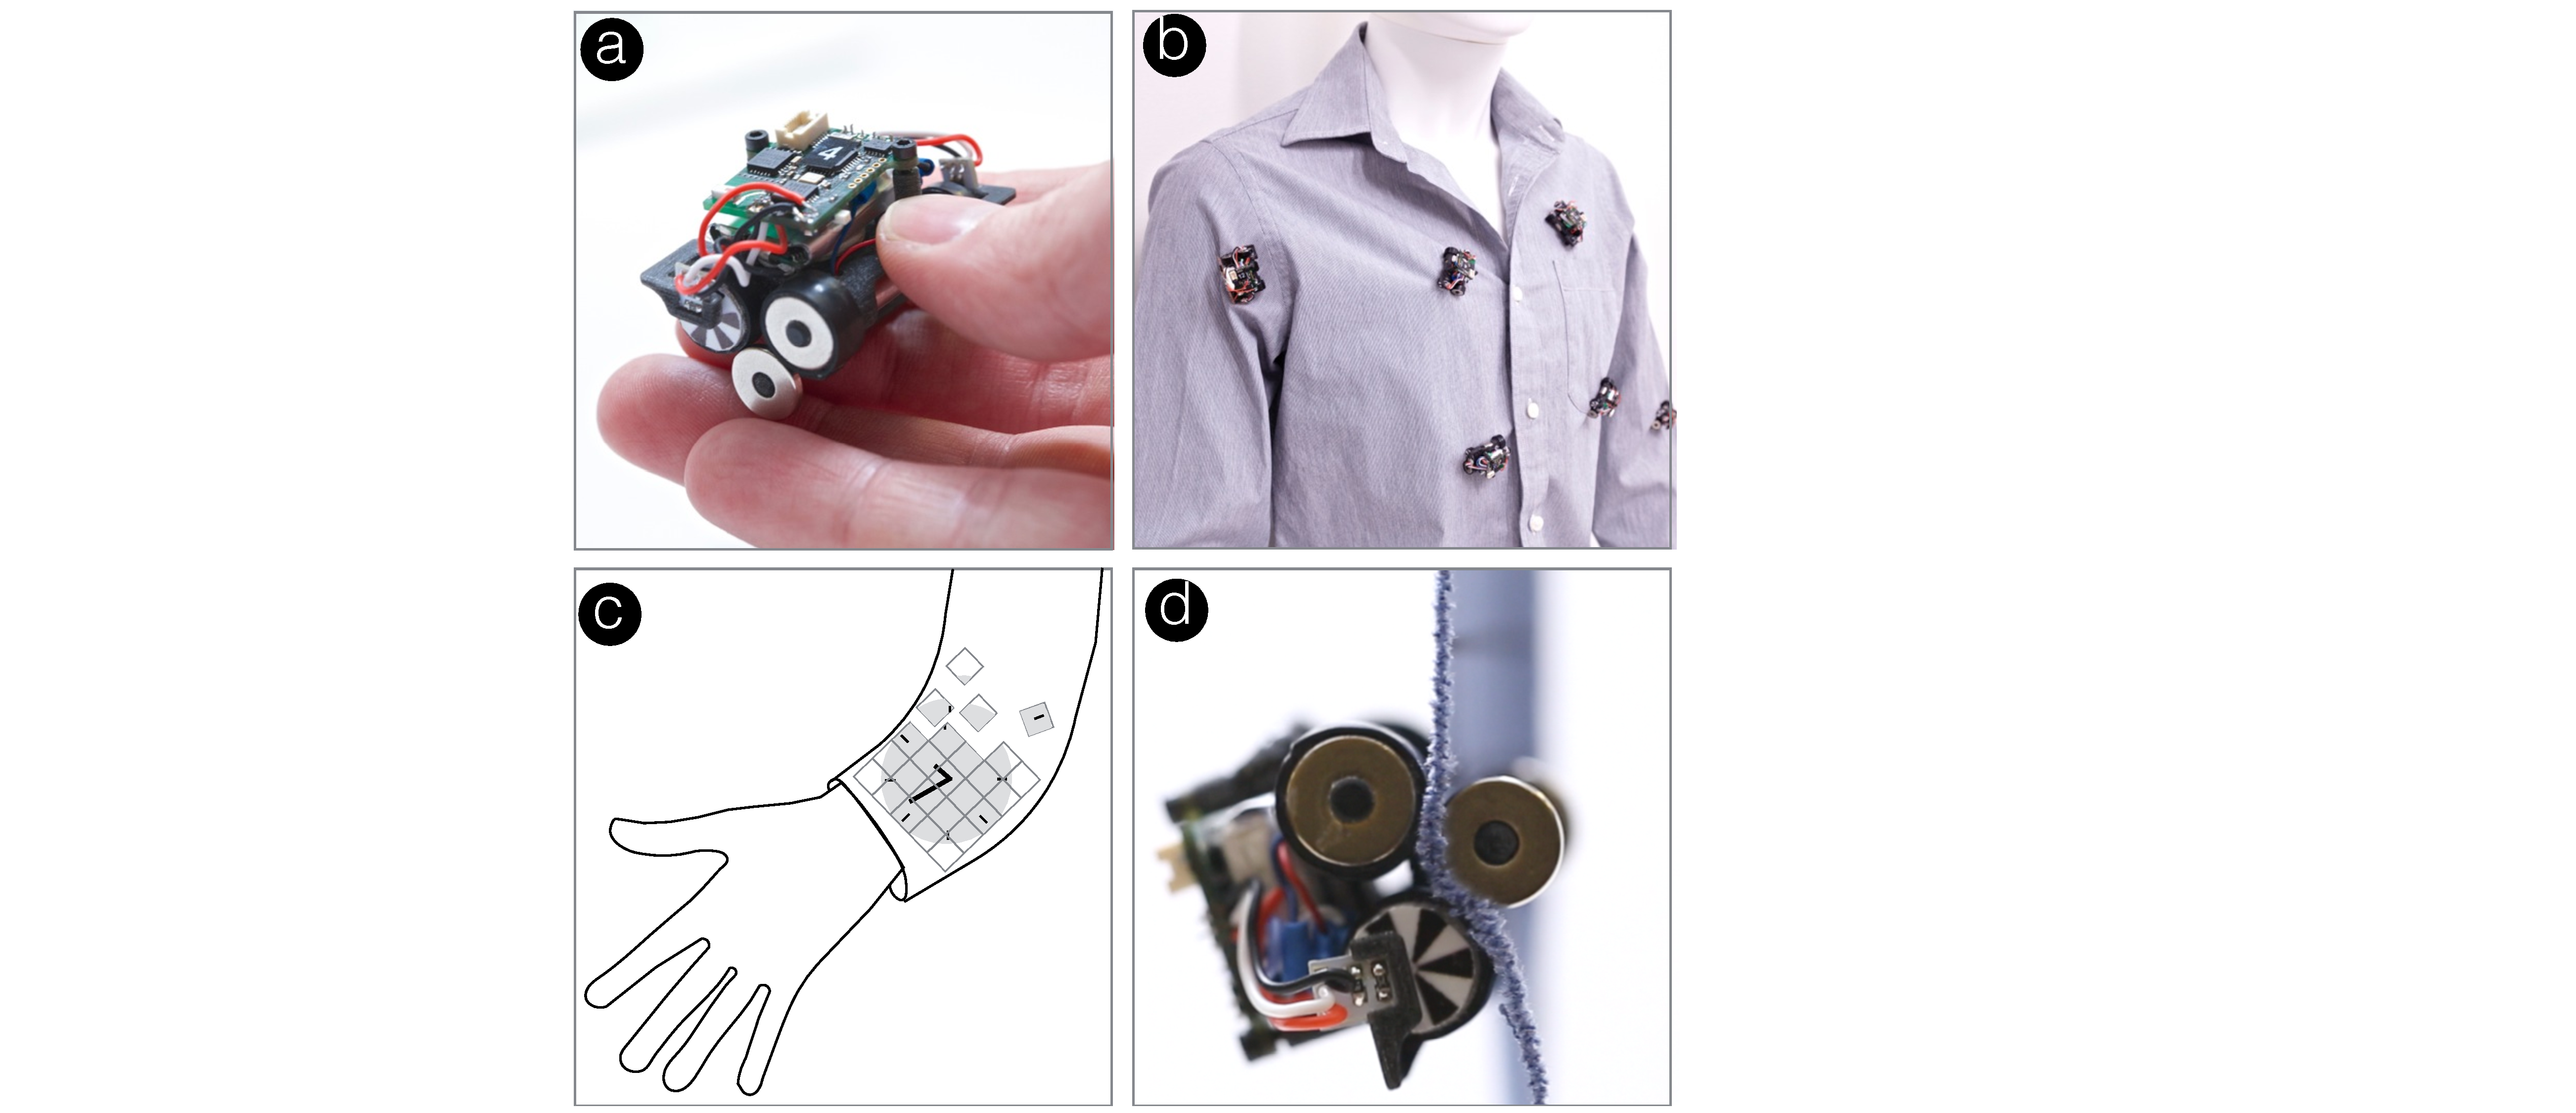
\includegraphics[width=10.0cm]{pictures/chapter4/front_pic_medium.pdf}
  \caption{a) Current Rovables prototype. Magnetic wheels provide an ability to climb vertical clothing. The onboard electronics and sensors provide autonomous operation. b) Multiple Rovables are climbing a shirt. c) In the future, Rovables could become fingernail sized. A swarm of them can create an on-body interface or do distributed sensing. d) Rovable climbing a vertical piece of fabric.}~
    \label{fig:front_pic}
\end{figure}

\section{Implementation}
In this section, we will describe the mechanical and electrical design of Rovables. All the design files will be open sourced at \href{http://github.com/rovables/}{github.com/rovables}



\begin{figure}[!h]
\centering
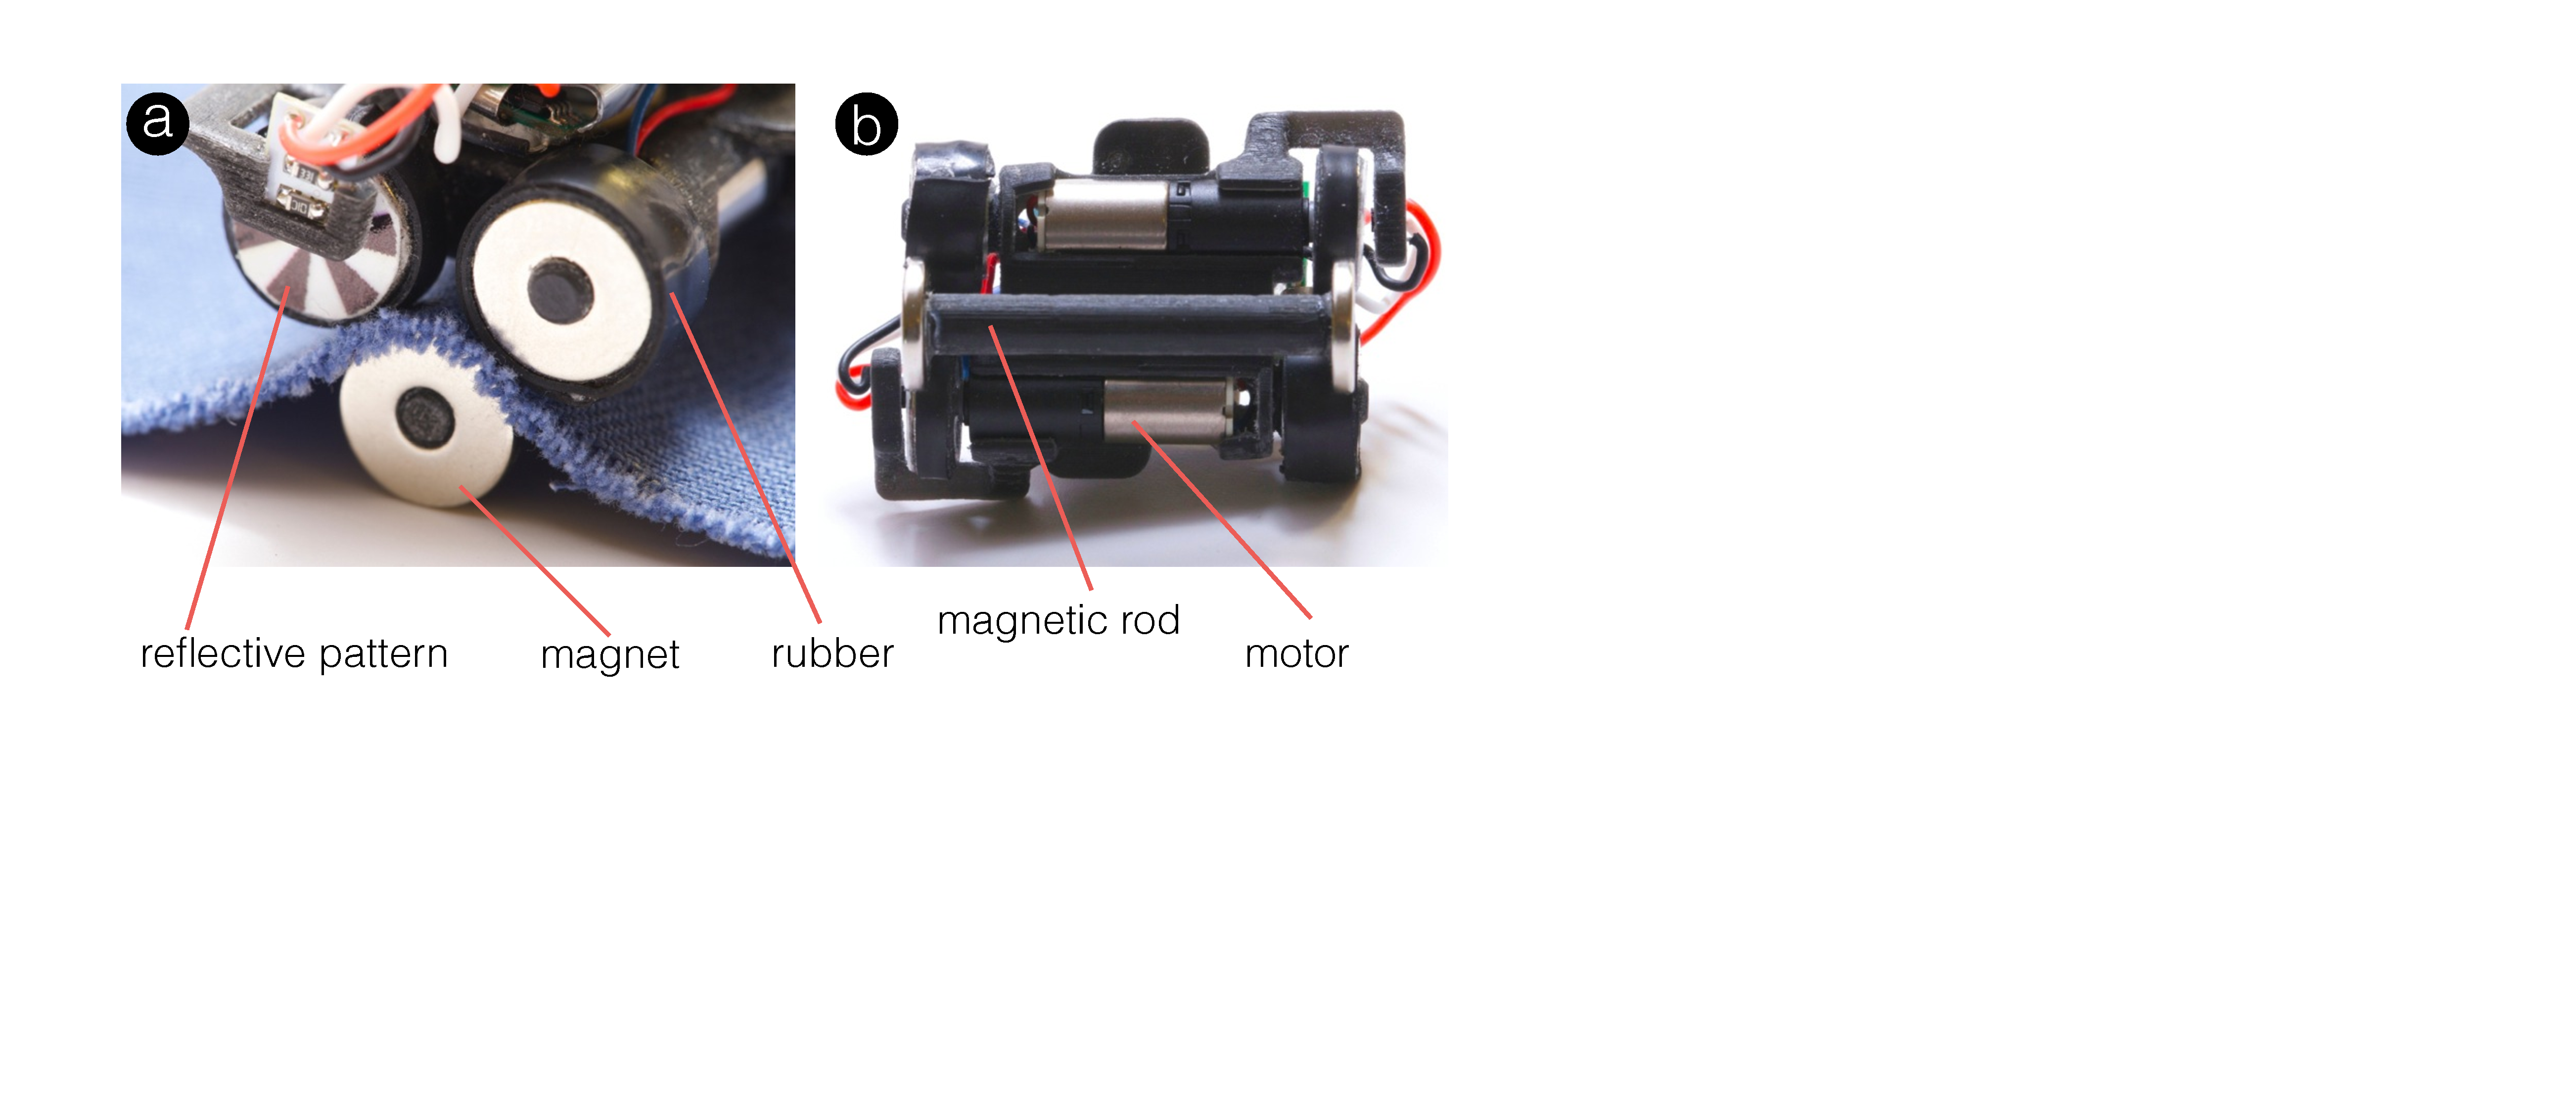
\includegraphics[width=1\columnwidth]{pictures/chapter4/drive_system.pdf}
\caption{Illustration of the magnetic drive system. a) The fabric is held between the top two wheels and magnetic rod on the other side. All the wheels are circular neodymium magnets. The reflective pattern on the wheels is used for the infrared encoder.  b) Underside view of the chassis, with the fabric, removed. Two motors are visible in this view.}
\label{fig:drive_system}
\end{figure}

\subsection{Cloth climbing}
The magnetic-drive chassis is shown in Figure~\ref{fig:drive_system}. We used two 136:1 planetary gear motors (TGPP06-D-136, TT Motor) for movement. Such motors are only 6mm in diameter and have a high gear ratio. The gear motors were attached to neodymium magnet wheels (9mm diameter). Next, to the drive wheels, another set of neodymium magnet wheels was used to stabilize the movement. Those wheels were connected by miniature ball bearings (4mm diameter), to reduce friction. Both sets of wheels were covered with 1mm-thick Neoprene rubber tires to reduce slippage. On the other side of the fabric, a rod with two neodymium wheels locked into the upper wheels. Because of magnetic attraction, the magnetic rod is moved with the upper wheels. This holds the robot in place, regardless of its orientation. The body of the robot was 3D printed in one piece using Objet Eden260VS (Stratasys) 

Other works used different mechanisms for climbing, such as by pinching the fabric~\cite{liu2012system}. Although our approach requires a magnet on the back side, we picked it for simplicity and ease of miniaturization.  

\begin{figure}[!h]
\centering
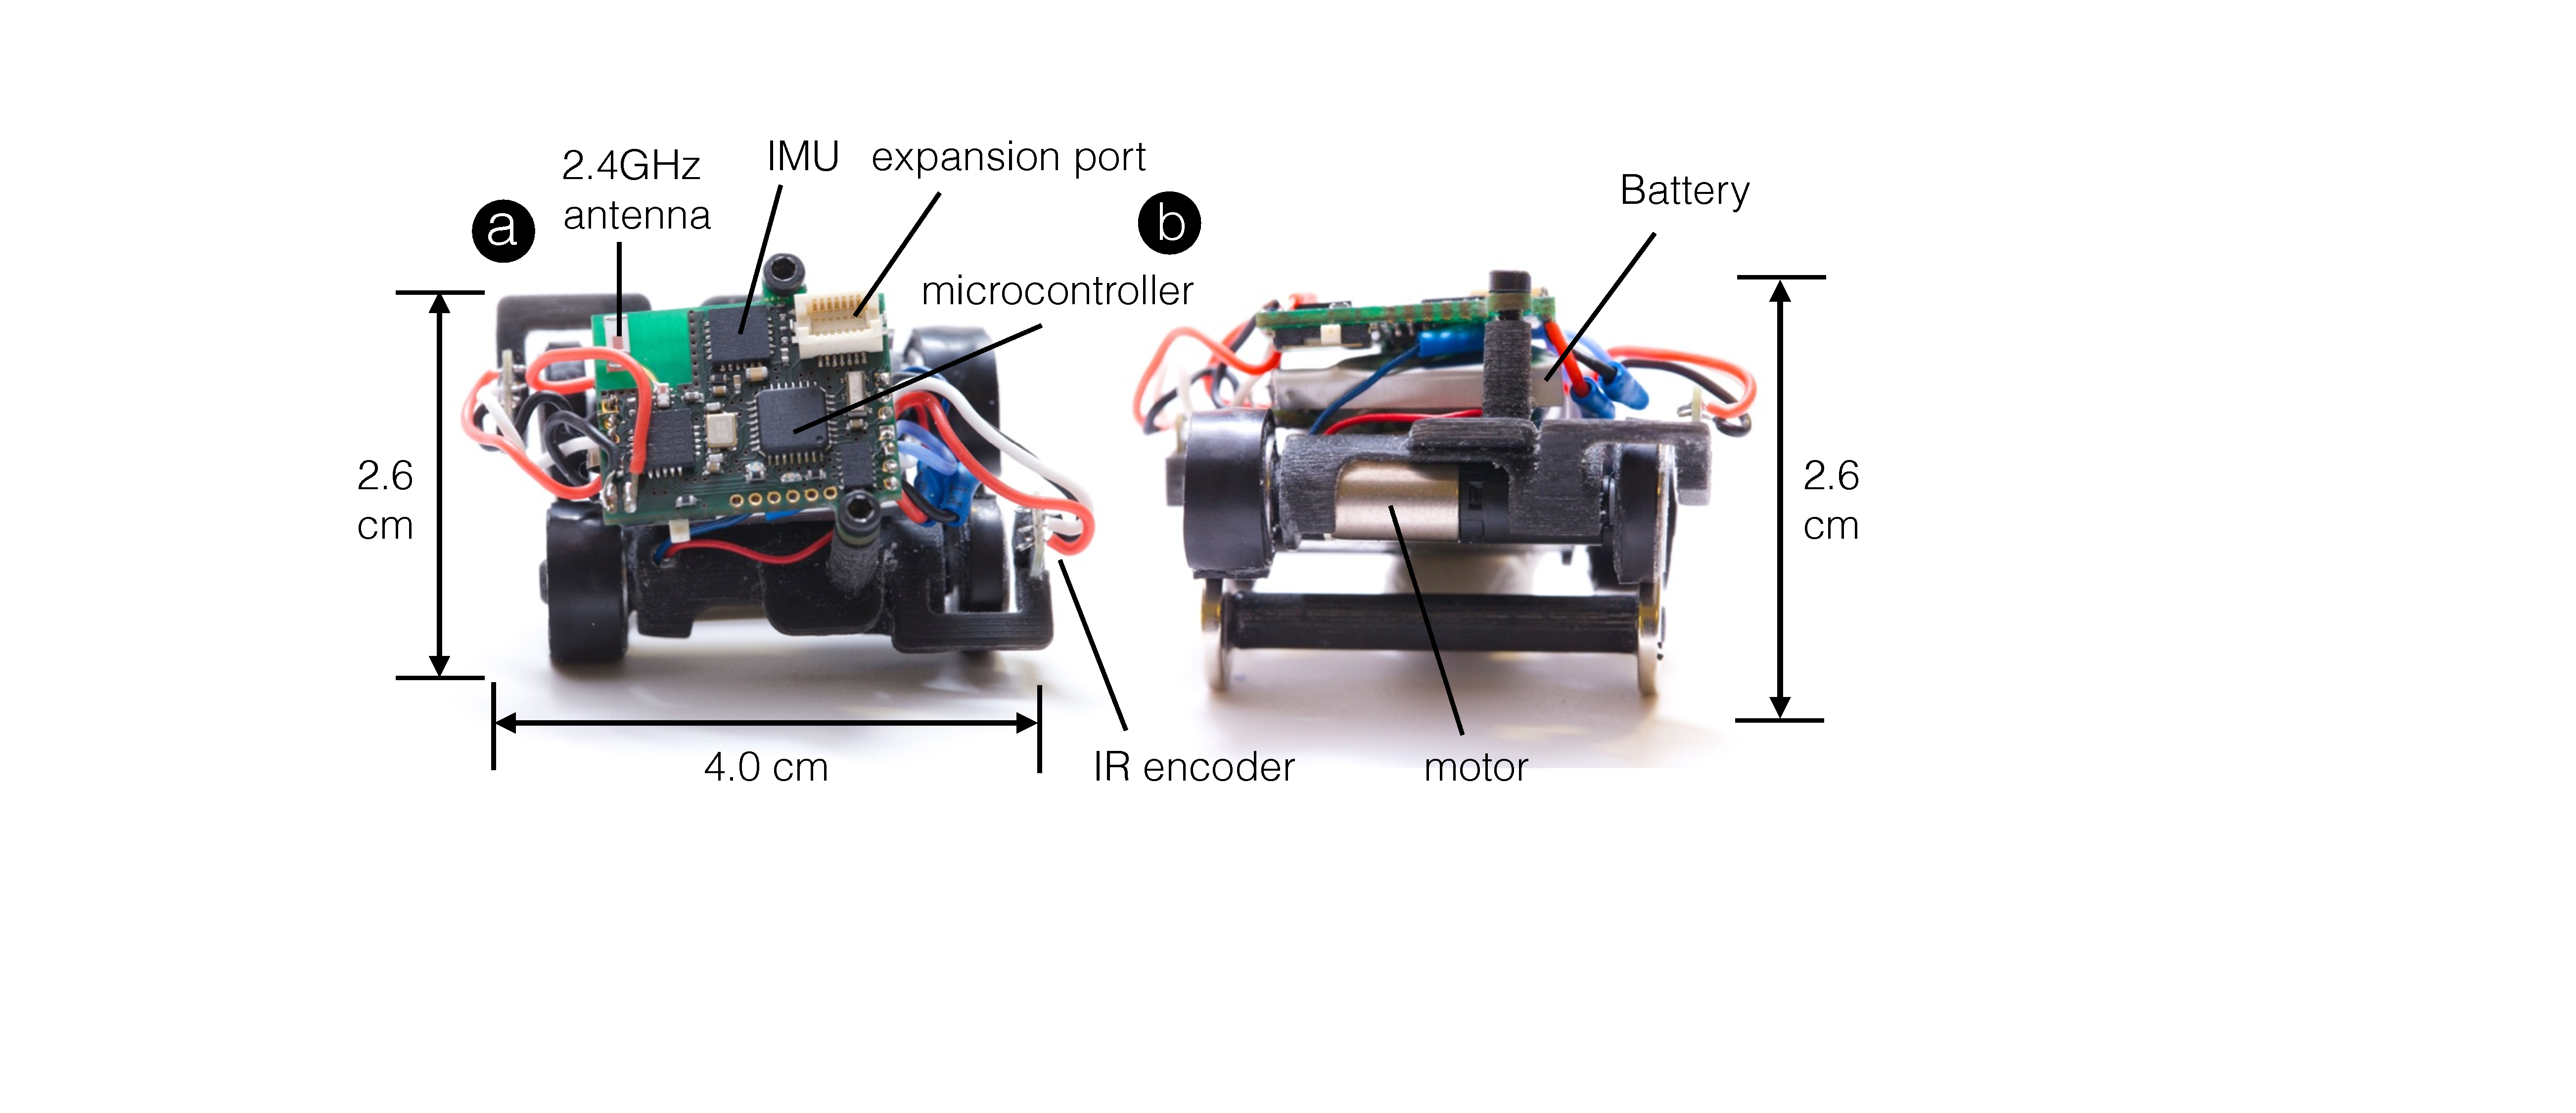
\includegraphics[width=0.8\columnwidth]{pictures/chapter4/top_side_view.pdf}
\caption{Picture of the electronics and sensors. a) Top view. The custom designed circuit board is visible on the top. Infrared encoders are placed on the left and right wheels. The expansion port on the top is used to add more functionality. b) Side view. As visible in this view, the battery is sandwiched between the motors and the circuit board. }
\label{fig:top_side_view}
\end{figure}

\subsection{Hardware}
The system diagram is shown in Figure \ref{fig:system_diagram}. To reduce the size and weight, we made a custom 1mm-thick PCB (printed circuit board), as shown in Figure~\ref{fig:top_side_view}. We added a 14-pin connector so shields can be added for more functionality (e.g., additional sensors). We exploit this feature in the applications section. The main processor is ATmega328p (Atmel). The system is powered by 100 mAh lithium polymer battery. 

For radio communications with the base station, we used 2.4GHz radio; nRF24L01+ (Nordic Semiconductors). We decided to use a custom wireless protocol versus standard (Bluetooth, WiFi) to allow control of multiple robots without significant latency while reducing power consumption. Furthermore, 2.4GHz frequency allowed for a miniaturized antenna. 
The base-station contained the same nRF24L01+ radio with extended range antenna. It also contained ATmega32u4 (Atmel) microcontroller to communication to PC over USB, and to control the radio. We used a server-client architecture for communications. On the PC side, C++ based openFrameworks was used to control Rovables, process and visualize data.  In this configuration, the base station is the server, and the robots are the clients. The robots send the data to the server at 10Hz intervals. To prevent data collisions with multiple radios the retry period was randomized for each robot. 

For orientation sensing, we used an MPU6050 (InvenSense) inertial measurement unit (IMU). It contains 3-axis gyroscope and 3-axis accelerometer and can calculate 3-D orientation onboard. To estimate the traveled distance and the speed, we designed incremental infrared optical encoders with GP2S60A (Sharp). The encoders work by measuring the changes in infrared reflectance of a disk with alternative white and black stripes. The disk was printed on glossy poster paper and glued on the wheels. To generate digital interrupts, the encoders were connected through a Schmidt trigger. We did not use magnetic encoders because of interference from magnetic wheels. For IR proximity sensing, four TSSP77P38 (Vishay) were used. The sensors were mounted on the removable display shield, which is further described in the applications section and Figure ~\ref{fig:displays}.

\subsection{Wireless Charging}
By putting an inductive coil (WR221230-36M8-G, TDK) on the undercarriage, Rovables can charge wirelessly. The coil is shown in Figure~\ref{fig:nfc_coil}. The coil is only 0.5 mm thick, so it does not interfere with movements. The charging was done using 13.56 MHz Qi wireless power standard. As a secondary purpose, the charger can serve as home, for the dead-reckoning system, described in the next section. When the device goes home, it can re-calibrate to reset the accumulated error. 

\begin{figure}[!h]
\centering
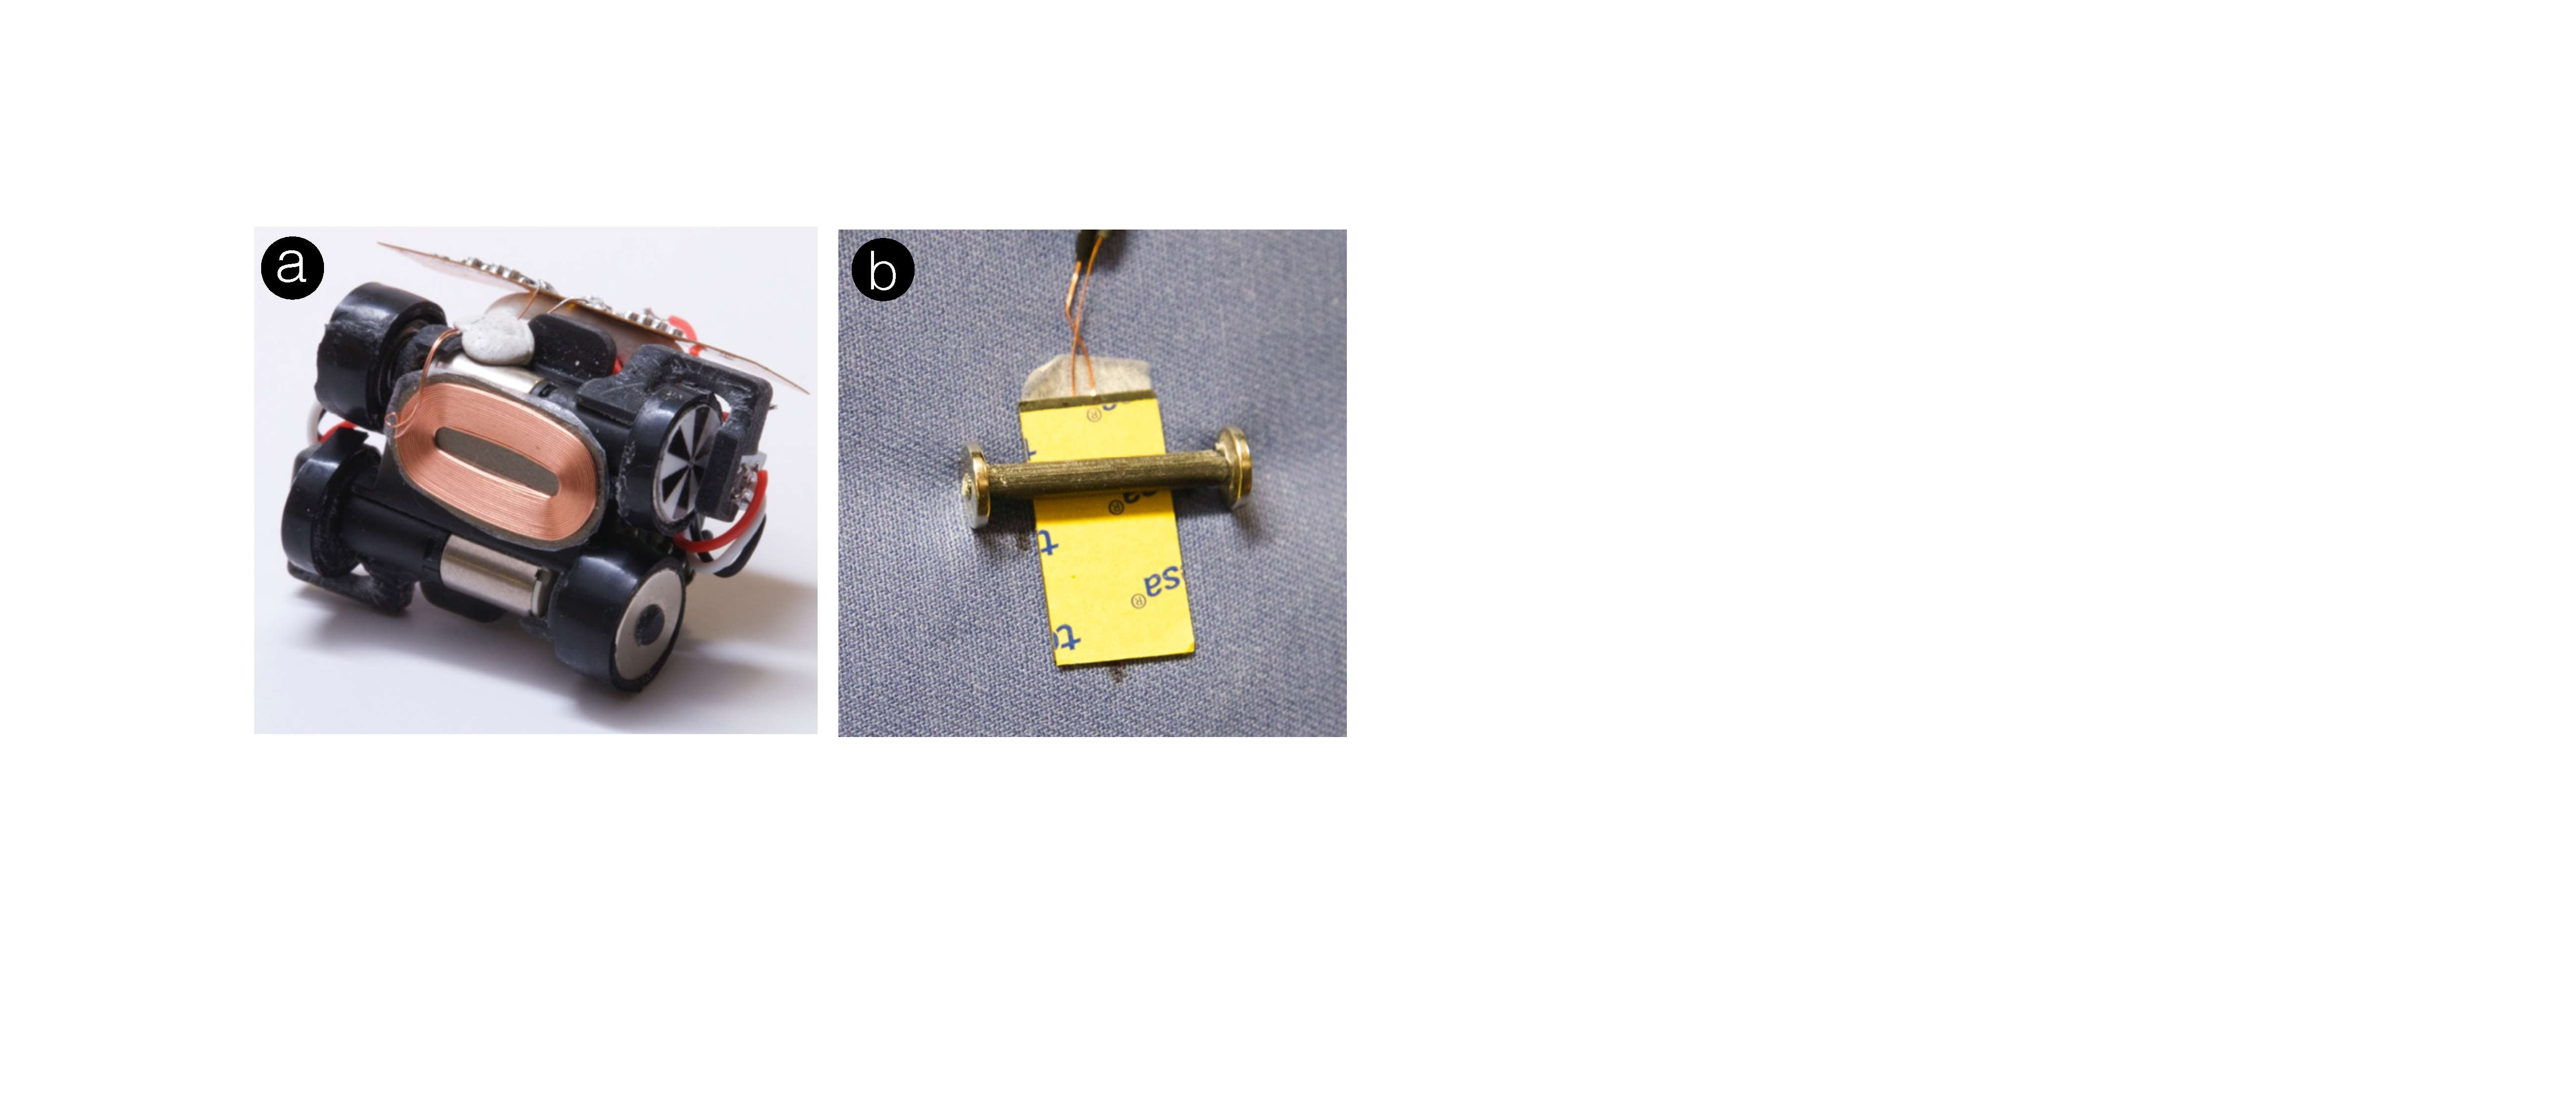
\includegraphics[width=0.8\columnwidth]{pictures/chapter4/nfc_coil.pdf}
\caption{The wireless charging system. a) The receiver coil is mounted on the underside of the chassis. b) The yellow transmitter coil can be taped on the back side of the fabric. The Rovable is parked on the coil, as seen by its magnetic rod. The main body is on the other side of the fabric.}
\label{fig:nfc_coil}
\end{figure}

\begin{figure}[!h]
\centering
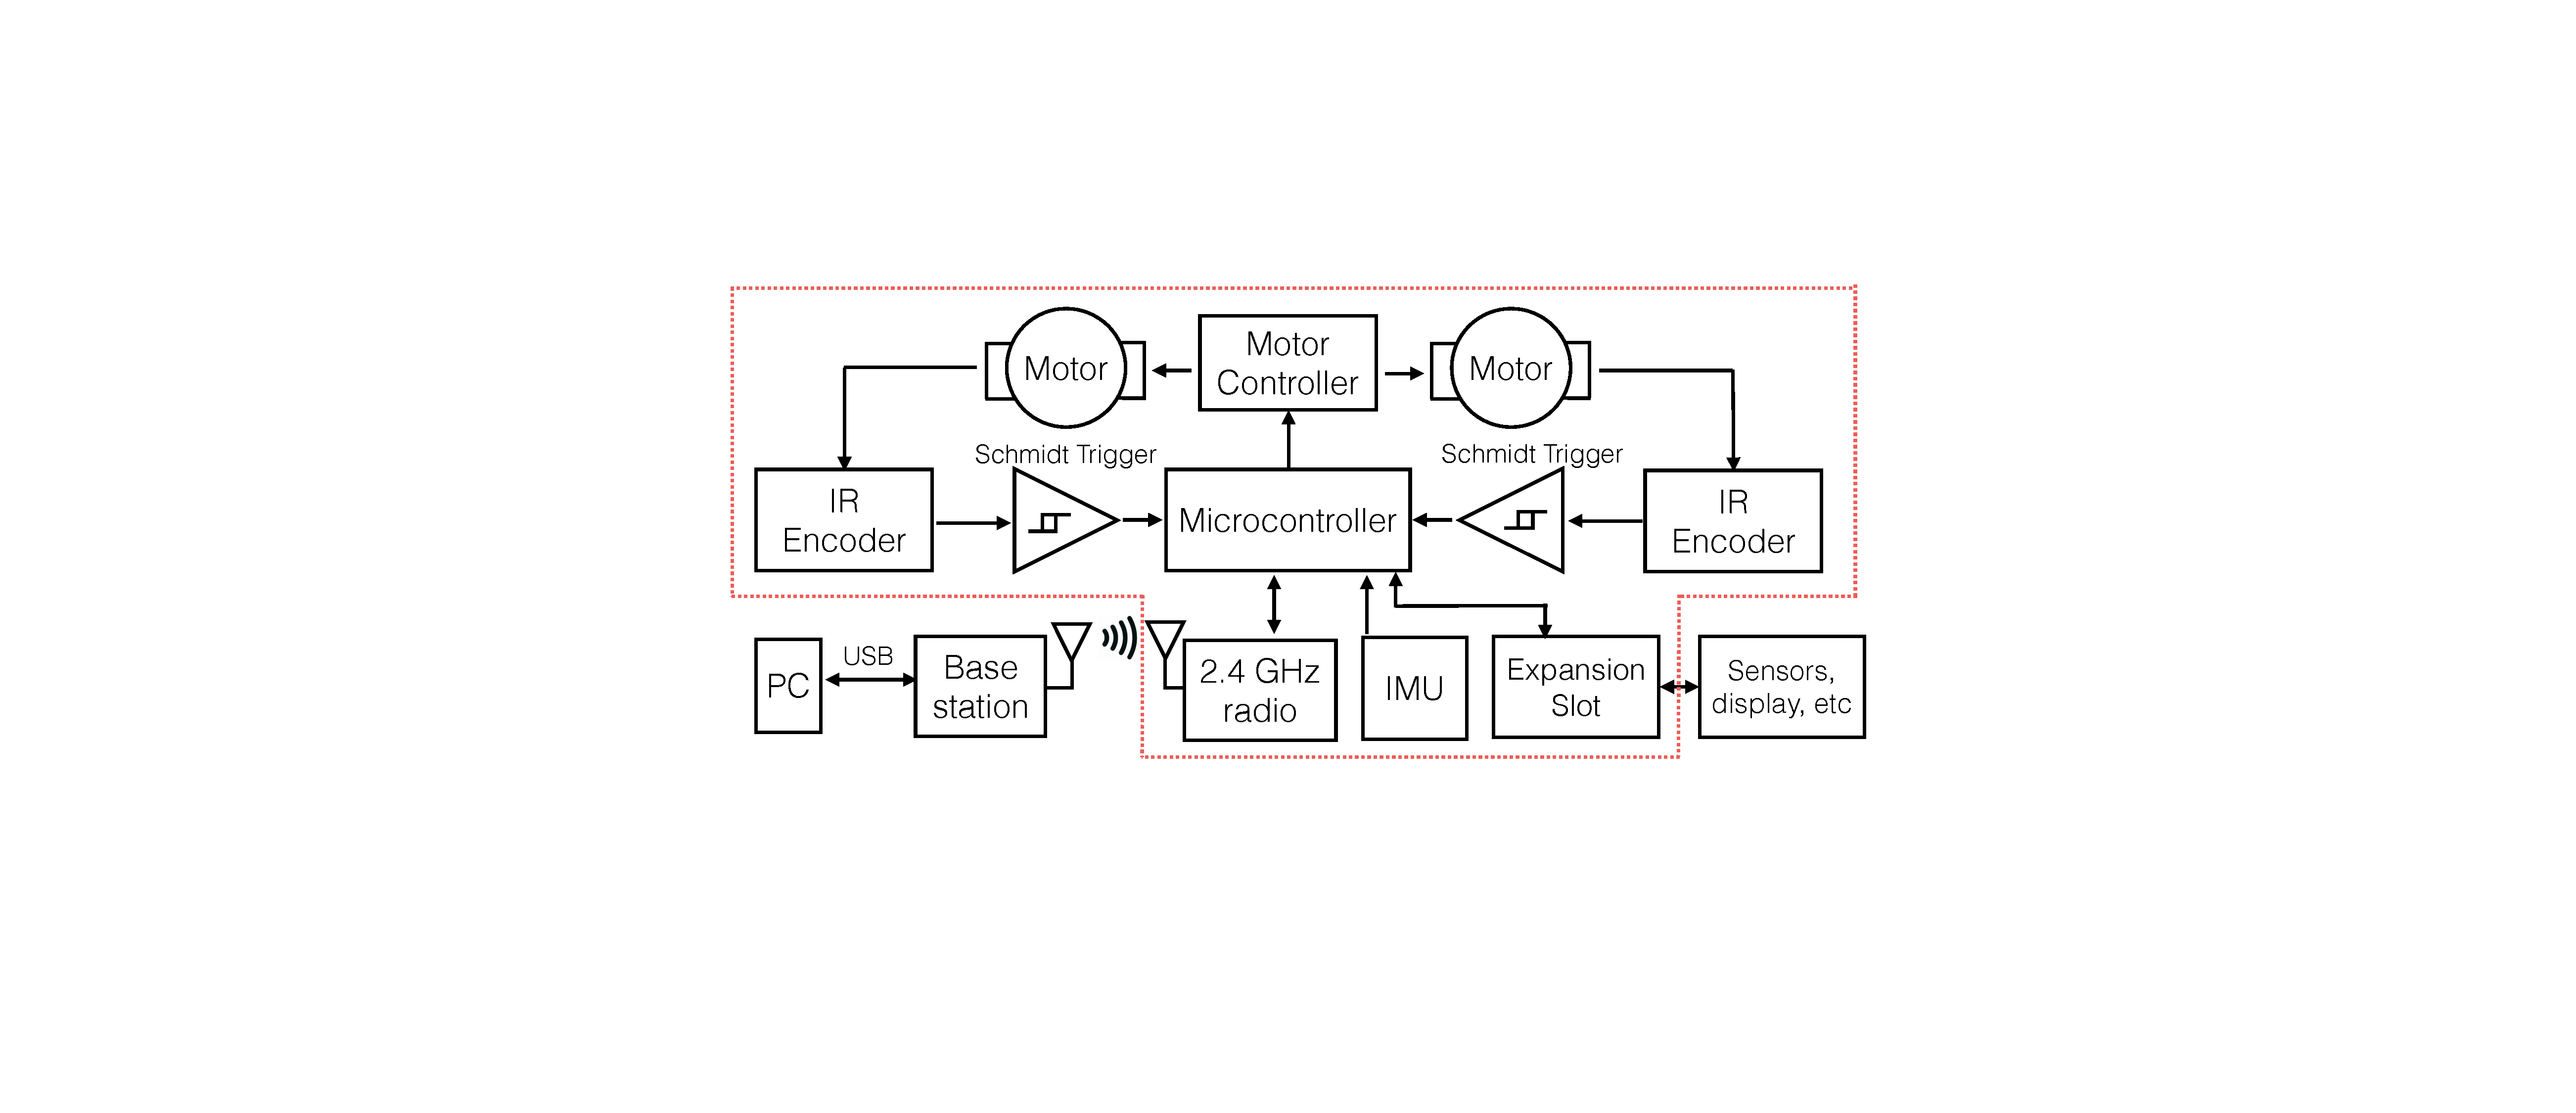
\includegraphics[width=0.8\columnwidth]{pictures/chapter4/system_diagram.pdf}
\caption{System diagram. The parts inside the red dashed lines are on the main board.}
\label{fig:system_diagram}
\end{figure}


\subsection{Wireless communications}
Each Rovable transmits and requests a 32-byte packet every 100ms, providing a data rate of 0.32Kb/sec. The network supports up to 3 robots reliably. With more robots, data collisions become more frequent and cause errors and high latency. In the future, collisions can be avoided with synchronization and by allocating transmissions into slots. 


\section{Summary}
This chapter described the implementation and design of Rovables. 
